Molecular structure originates from the underlying architecture of atoms, governed by quantum mechanical principles. Electrons are not treated as point particles following classical trajectories, but as wavefunctions — mathematical objects encoding the probability distribution of their position in space. The behavior of an electron is determined not by Newtonian forces but by the solutions to the Schrödinger equation, which defines discrete energy levels and corresponding spatial distributions.

The time-independent Schrödinger equation relates the system's total energy to its spatial properties: $\hat{H}\psi = E\psi$, where $\hat{H}$ is the Hamiltonian operator, $\psi$ is the electron wavefunction, and $E$ is the energy eigenvalue. These quantized solutions stand in sharp contrast to the continuous energy spectra predicted by classical mechanics and form the basis of modern atomic theory. Each solution defines an orbital, characterized by specific energy, shape, and nodal structure. In hydrogen, the $1s$ orbital is spherically symmetric, while higher orbitals — $p$, $d$, and $f$ — exhibit directional lobes and angular nodes arising from quantum mechanical constraints.


\begin{figure}[H]
\centering
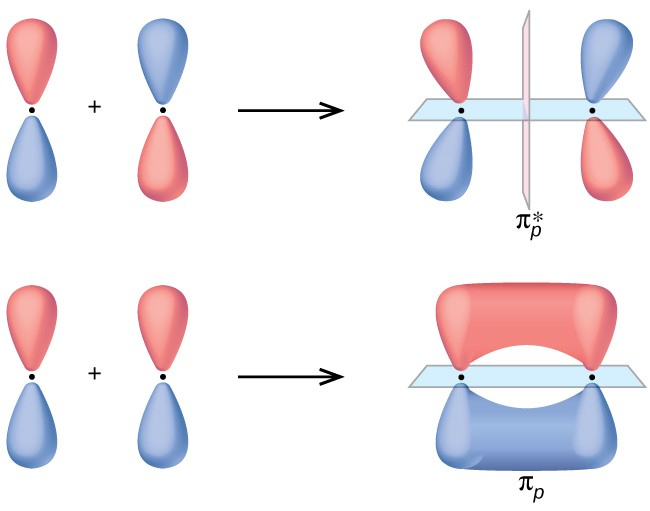
\includegraphics[width=0.7\textwidth]{46_WoodwardHoffmannRules/CNX_Chem_08_04_pMOpi1.jpg}
\caption{Formation of $\pi$ and $\pi^*$ molecular orbitals from lateral overlap of $p$ orbitals. Bonding $\pi_p$ orbitals (bottom) feature electron density above and below the internuclear axis. Antibonding $\pi_p^*$ orbitals (top) exhibit a nodal plane and out-of-phase lobes. Adapted from OpenStax Chemistry, Section 7.8: Molecular Orbital Theory. Licensed under CC BY 4.0.}
\label{fig:pi_p}
\end{figure}

When atoms bond to form molecules, their atomic orbitals combine into molecular orbitals that extend across multiple nuclei. Constructive interference between wavefunctions produces bonding orbitals, concentrating electron density between nuclei and stabilizing the system. Destructive interference leads to antibonding orbitals, characterized by a nodal plane between nuclei and elevated energy. The occupation of these orbitals follows the Pauli exclusion principle: electrons fill available molecular orbitals from lowest to highest energy, pairing spins where necessary. This filling determines the molecule’s electronic ground state and dictates its chemical reactivity.

\begin{figure}[H]
\centering
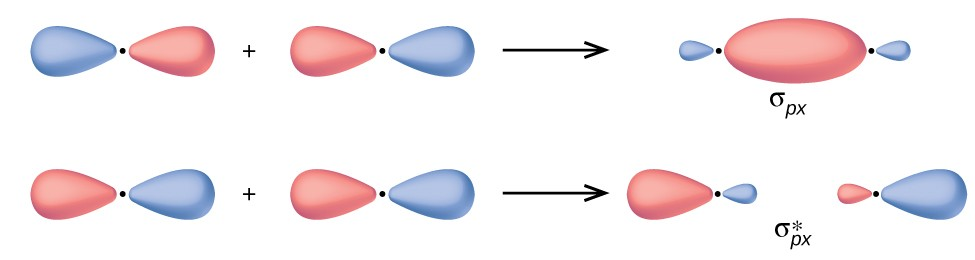
\includegraphics[width=0.85\textwidth]{46_WoodwardHoffmannRules/CNX_Chem_08_04_pMOsigma1.jpg}
\caption{Formation of $\sigma$ and $\sigma^*$ molecular orbitals from head-on overlap of two $p_x$ atomic orbitals. Constructive interference (top) yields a bonding $\sigma_{p_x}$ orbital. Destructive interference (bottom) yields an antibonding $\sigma_{p_x}^*$ orbital. Adapted from OpenStax Chemistry, Section 7.8: Molecular Orbital Theory. Licensed under CC BY 4.0.}
\label{fig:sigma_px}
\end{figure}

Organic chemistry is dominated by molecules composed of carbon, hydrogen, oxygen, and nitrogen. Carbon’s tetravalency, enabled by $\mathrm{sp}^3$, $\mathrm{sp}^2$, and $\mathrm{sp}$ hybridizations of their $s$ and $p$ orbitals, allows the formation of stable $\sigma$ and $\pi$ bonds in chains, rings, and three-dimensional networks. $\pi$ bonds, arising from lateral overlap of unhybridized $p$ orbitals, are more diffuse than $\sigma$ bonds and more sensitive to molecular geometry. In conjugated systems, $\pi$ bonds alternate with $\sigma$ bonds, allowing electron delocalization across multiple atoms. This delocalization lowers the system's energy and imparts distinctive electronic, optical, and chemical properties.

Conjugated $\pi$ systems underpin many organic processes, including pericyclic reactions. These reactions proceed concertedly: all bond-making and bond-breaking events occur simultaneously in a single kinetic step, without discrete intermediates. The hallmark of pericyclic reactions is cyclic electron flow, with electrons moving around a closed loop and the reaction passing through a highly ordered, often symmetric transition state. The feasibility and stereochemical outcome of these reactions depend critically on the phase relationships and symmetries of the participating molecular orbitals.

The Schrödinger equation not only governs the existence of orbitals but also constrains their behavior under chemical transformation. The molecular Hamiltonian $\hat{H}$ is invariant under the symmetry operations of the molecule — rotations, reflections, and inversions that leave the nuclear arrangement unchanged. Consequently, the eigenfunctions of $\hat{H}$ — the molecular orbitals — must transform deterministically under these operations. During a reaction, maintaining continuous orbital symmetry is essential for preserving low-energy pathways; symmetry-forbidden distortions introduce high energy barriers or render the reaction inaccessible.

In 1965, Robert Woodward and Roald Hoffmann formalized these symmetry considerations into a predictive theory now known as the Woodward–Hoffmann rules. Their insight was that the feasibility of pericyclic reactions can be determined by analyzing how the occupied molecular orbitals evolve along the reaction coordinate. If symmetry is preserved throughout the transformation, the reaction is allowed; if symmetry is disrupted, the reaction is forbidden under the given conditions.

The rules distinguish between thermal and photochemical activation. Under thermal conditions, reactions involve the ground electronic state, and the correlation of the highest occupied molecular orbitals (HOMOs) of reactants and products determines the pathway. Under photochemical conditions, excitation promotes an electron into a higher orbital, altering symmetry relationships. The relevant correlation then involves the frontier orbitals of the excited state. In both cases, the requirement is continuous, symmetry-allowed transformation of the electron configuration.

Electrocyclic reactions exemplify the application of the Woodward–Hoffmann rules. In the thermal ring closure of butadiene (four $\pi$ electrons), the terminal $p$ orbitals must rotate conrotatorily — both twisting in the same direction — to preserve orbital symmetry and achieve constructive overlap. In contrast, the thermal ring closure of hexatriene (six $\pi$ electrons) proceeds through disrotatory motion, with terminal $p$ orbitals rotating in opposite directions. Photochemical activation reverses these patterns: butadiene closes disrotatorily, and hexatriene closes conrotatorily.

Cycloadditions provide another domain where the rules manifest with precision. In the Diels–Alder reaction, a [4+2] cycloaddition involving six $\pi$ electrons, the suprafacial-suprafacial overlap of the diene and dienophile frontier orbitals is symmetry-allowed thermally. Conversely, a [2+2] cycloaddition, involving two alkenes and four $\pi$ electrons, is thermally forbidden due to phase mismatches but becomes allowed under photochemical conditions, where excitation modifies the symmetry properties of the participating orbitals.

Sigmatropic shifts extend the theory further. These reactions involve the migration of a $\sigma$-bonded group across a conjugated $\pi$ system. The symmetry of the transition state, visualized through correlation diagrams, dictates whether the shift is thermally allowed. For example, the [1,5]-hydride shift proceeds thermally because the orbital interactions preserve bonding symmetry throughout the migration.

The Woodward–Hoffmann rules reveal a connection between quantum mechanics and chemical reactivity. They show that chemical transformations are constrained by the abstract properties of wavefunctions: symmetry conservation is not an empirical observation, but a mathematical necessity stemming from the invariance of the Schrödinger equation under molecular symmetries.

The scope of the rules extends beyond synthetic chemistry into biological systems. In rhodopsin, the light-sensitive pigment of the retina, photoisomerization of the retinal chromophore exemplifies a pericyclic process governed by symmetry. In its ground state, thermal isomerization is symmetry-forbidden and thus extremely rare, preserving visual sensitivity. Upon photon absorption, the excited-state symmetry allows rapid, concerted isomerization from the 11-cis to the all-trans configuration, triggering visual signal transduction.

Even pathological processes, such as the formation of toxic byproducts in age-related macular degeneration, can be interpreted through the lens of orbital symmetry. Under oxidative stress, reactive intermediates enable cyclizations that would otherwise be forbidden thermally. The Woodward–Hoffmann rules thus provide an insight not only for predicting reaction diagrams but understanding larger systems based on the underlying molecular logic.
\newpage
\begin{commentary}[Mathematical Abstraction as Physical Constraint]
What makes the Woodward–Hoffmann rules particularly striking is not merely their utility, but their origin. They derive from abstract properties of the Schrödinger equation — specifically, the requirement that its solutions respect the symmetries of the Hamiltonian. This is not an empirical rule, nor was it designed to explain organic reactivity. It is a consequence of a mathematical formalism developed to account for atomic behavior on quantum scales.

Yet that same formalism — often regarded as remote or epistemologically distant — reappears here as a governing principle for chemical structure, stereochemistry, and biological function. The orbital symmetries that dictate reaction outcomes are not empirical regularities forced into a model; they are constraints embedded in the mathematical theory. When that mathematics was extended into molecular systems instead of requiring adjustment — it revealed new regularities that had previously been invisible. This constitutes an unusual kind of scientific success in which too often rules are retrofitted to explain the data. 
\end{commentary}
